

\section*{Selection of 3D Evironment}

The key decision before implementation could commence was the environment
to work in. This was heavily inter-linked with the choice of main
programming language. Due to time constraints building an entire 3D
engine would be outside the scope of the project.


\subsection*{Programming Language Considerations}


\subsubsection*{C++}

Designed to be a superset of the C language, supporting the object-orientated
paradigm. It is industry standard for almost all 3d graphics development
(BIB http://gamearchitect.net/Articles/WhyC++.html), bridging the
gap between lower level languages such as C and object orientated
languages such as Java and C\#. Due to its speed and power combined
with available 3d libraries and very high portability if considering
the merits of languages alone this would have been the easy choice!
The majority of available engines are also written in the language
offering a large selection when it came to this.

However as a team we had no experience at all with the C++ programming
and at the time of selection only a minor knowledge of C. This alone
would be a steep learning curve, but to provide the 3d environment
required an understanding of either the OpenGL library or Direct3d
(See Graphics Standards Below) would have possibly also been required.
There are also those who argue instead of trying to bridge gaps, low
level components of games should be written in C. They argue due to
the information hiding afforded by C++ it is often easier to write
efficien code in its lower level counterpart!(BIBX http://gamearchitect.net/Articles/WhyC++.html)
Memory management is also far less advanced than alternatives offering
an easy leeway to memory leaks.


\subsubsection*{Java}

Written to have as few implementation dependencies as possible java
is incredibly portable (BIB http://www.java.com/en/about/). Rather
than to binary java compiles to what is known as bytecode which runs
on the Java virtual machine unrelated to the architechture underneath.
The language as with C++ implements the object-orientated paradigm
allowing abstraction and with standard extentions such as Java3D offers
a less intimidating entrance into 3D.

With astonishingly powerful free IDE's such as Eclipse and Netbeans
writing in Java becomes quick and painless. Threading is built in
and whilst large the instruction set is easy to learn. To add to this
Java is the language we as a team have the most experience with. This
would allow implementation of the basic components to begin immediately.
There is also the java garbage collector. This automatically retrieves
memory which is no longer reachable taking away risks of memory leakage.

The downside to Java is the abstraction from architechture comes at
a cost of speed. Since there is both virtualisation combined with
a high level environment things are far from efficient (BIB Jelovic,
Dejan. ``Why Java Will Always Be Slower than C++''). 


\subsubsection*{Python / A high level scripting language}

The majority of performance issues relating to 3D programming come
from the underlying engine. Since we were anticipating usage of a
preexisting system, we could then build our system over the top of
this using a high level language such as Python. Using libraries such
as Boost.Python (BIB http://www.boost.org/doc/libs/1\_40\_0/libs/python/doc/index.html)
the two languages can be bound allowing claimed seemless interoperability.
Performance bottlenecks due to Python could be overcome using C++.
Less critical tasks could be written quickly and easily in Python.

With some team Python experience combined with a less intense learning
path than pure C++ this methodology was a strong consideration.


\subsection*{Graphics standards}

Whilst this mostly came down to our choice of engine, it was a consideration
to take during our decisions. There are only really two options, Direc3D
and OpenGL.


\subsubsection*{Direct3D}

Direct3D is a proprietry API (GLOS) designed by Microsoft Corporation.
It was created to allow games creators more open access towards hardware
giving much better performance. Whilst in previous years it suffered
performance issues and multiple bugs it has improved drastically and
is now considered by many to be the industry standard for Windows
platforms (BIB http://www.gamedev.net/page/resources/\_/technical/graphics-programming-and-theory/direct3d-vs-opengl-which-api-to-use-when-whe-r1775).

Its power is also one of its key weaknesses. There is a steeper learning
curve than OpenGL and it takes considerable work just to initialize.
The other big weakness is portability. Outside of windows support
is extremely poor. Whilst Wine, a compatability layer for Unix based
systems offer mostly functional ports these are impeded due to dependencies
on other Windows libraries.


\subsubsection*{OpenGL}

OpenGL is an open standard API which was for a number of years little
disputed as the industry standard. It is available on a large variety
of platforms including Windows, Mac \& Linux based systems. It provides
a strong range of functionality and was designed to be as futureproof
as possibly. There is a proven history of stability and to add to
its core functionality there is the ability for extentions. Since
its future is controlled by a board made up from a large diverse group
of companies its strengths apply to a large number of applications.

Downsides are also many but revolve around two main issues. OpenGL
was built 10 years ago and the future is was built to work for as
arguably come and gone. Extensions go a way to remedy this but are
hindered by many being vendor specific.

Code can also be incredibly messy, again partially down to extensions.
Often one function can have over a dozen names!


\subsection*{3D Engines}

The majority of the 3D functionality we needed could be provided by
an existing engine, either developed for simulation or game purposes.
Concepts required are needed by a wide range of industries making
current developments extensive and abundant.

Due to time constraints it would be incredibly difficult to create
a bespoke system able to provide as detailed and efficient performance.
As a result of this we decided to use one of these pre-existing solutions.
This choice would be heavily interlinked with our preferences towards
other tools.

Many of these are actually games engines. Games engines often are
designed to simulate a real-world environment which offers exactly
what is needed for this project. Due to the copious options available
only a subset are mentioned below.


\subsubsection*{Unity }

Unity is a cross platform engine written in C/C++, however it also
supports code written in C\# and javascript. It has its own rendering
capable of using Direct3D or OpenGL. There is strong support for 3D
model importation from a large range of formats. It has its own scripting
language as well as supporting C\# and Boo (which has a syntax inspired
from Python). The basic liscense would provide all the features we
needed and is free.

Unitys strengths are also the reasons not to use it for a large crown
based simulator. The emphasis is on providing incredibly powerful
GUI graphical design tools got games. The logic is aimed to be done
entirely in scripting languages which would give performance issues
when combined with the behavioural processing we would require.

Whilst C\# can be used we have no experience with the language. Whilst
its similarities to Java would allow a short learning period it then
asks why we wouldn't just use Java in the first place. C\# as with
Java offers performance shortfalls when compared to C/C++.


\subsubsection*{Panda3D}

Panda3D is an open source framework for 3D rendering and development
of programs written in Python and C++. It offers a reasonably powerful
environment with a relatively shallow learning curve. There is a strong
and active community support system but the documentation appears
to be lacking compared to other alternatives.

The platform is cross platform among the three key operating systems.
It supports both OpenGL and Direct3D providing a relatively thin wrapper
around the lower level API's.

If we decided to take the Python and C++ route this would be a stong
option to consider.


\subsubsection*{jMonkey Engine}

jMonkey is designed partially as a games engine and partially as a
replacement for the now unsupported Java3D. Written purely in Java
all the advantages mentioned towards the language above would also
apply here. All recent versions of OpenGL are also fully supported
offering advanced graphics capabilities.

Fundamentaly the project is solely a collection of libraries making
it a low-level tool which would give us the flexibility we would need
considering the majority of our code would be related to the simulation
as opposed to the graphics rendering.

If we were to decide to work in Java there was no comparable competition.


\subsubsection*{CryENGINE 3}

CryEngine is an advanced engine created by Crytek originally as a
technology demo for NVidia but the company soon saw its potential.
This has led to massive success with a burst of successful high profile
games based on the engine.

Programming for CryEngine is done using C++. This gives an extremely
powerful combination allowing incredible graphics with a high performance
back end.

The big downside is the lack of support for OpenGL. As a result there
is little portability outside of Windows. It is also only free for
non-commercial use, meaning if the project were to be taken beyond
the initial research aims an incredibly expensive liscence would be
required.


\subsubsection*{Game Blender}

Blender is a free and comprehensive 3D production suite, one component
of which is a games engine. Considering Blender was a strong contender
for use in our modelling (See Modelling below) there would be no importation
issues. The engine is a mostly independent component written in C++
including support for Python scripting. Whilst a relatively young
project it offers all the 3D functionality that would be required,
however is lacking in the back-end code support we would need.


\subsection*{3D Modelling}

To manipulate a 3D environment we needed to first create one! This
involved modelling the chosen structure in a way that could be imported
into the physics engine. Since many of the engines considered included
modellers again this decision was somewhat linked to that decision.

\subsubsection{How the model progressed}
Figures 2, 3, 4, and 5 in section shows blueprints of each deck: Weather Deck, Tween Deck, Lower Deck and Cargo Hold respectively.
\begin{center}
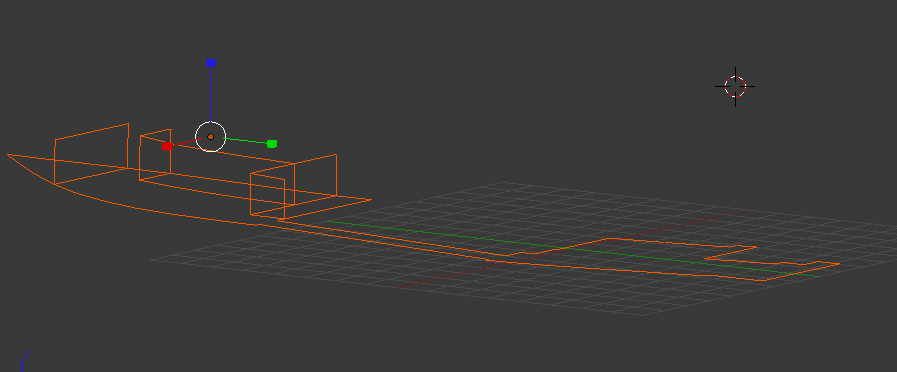
\includegraphics[scale=0.5]{../images/deck.png}
\\layer of deck
\end{center}
Each blueprint is used as a model to build a ship starting from the lowest to top deck and it is modelled individually using Blender layer.
To make curvatures matched to the floors accurately, cross sectionals is used so model scaling can be seen easily.
It is difficult to model a ship hull using only cross sectionals because its shape is round and consists of two or more profiles.
Therefore, skinning is applied (the fine art of defining a surface using more than one profiles).
In blender, skinning can be adopted by preparing as many curves of the desired shape and then converting them to a single NURBS(Non-Uniform Rational B-Spline) 
surface.


\subsubsection*{Blender}

As mentioned above Blender is a comprehensive 3D production suite.
Its main usage is in creation of 3D models. A large number of the
games engines we were considering either supported Blenders native
.blend format, or one of the many alternative formats the suite could
export as. There is extensive documentation combined with a strong
and active support community.

The featureset offered is comparable with some of the widespread industry
tools. Released under a GNU General Public License the software is
free for all usage. We also have some basic experience with the package.


\subsubsection*{Autodesk 3DS Max}

3DS Max is an incredibly powerful suite and the one most used in the
modelling industry. Comprehensive and versatile but the features come
at a cost. Lisenses are extremely expensive and the system requirements
are far from low. Whilst the liscence cost can be avoided since free
versions are available for students, we would need to gain access
to hardware capable handling the software.


\subsubsection*{Hexagon}

Hexagon unlike the other options discussed is purely a modelling program.
Offering equal functionality in this area advanced and detailed models
can be built. The interface is intuitive and easy to learn. The software
also has a very low retail price.


\subsection*{Choices}

Whilst the Python and C++ routes were a strong consideration it was
decided the benefits failed to overcome the time required to learn
a completely new language. Although documentation was far from perfect
jMonkey appeared to offer all the features we required. It was decided
that provided the back-end code was written in a reasonably efficient
manner performance should not be an issue.

Since jMonkey offered an inbuilt importation Blender was a complimentary
modelling choice. The minor benefits offered by the proprietary solutions
were far from counterbalancing the restrictions liscenses would incur.


\section*{Project Management}


\subsection*{Project Management}

For a project of this scale to be successful there needs good and
common communication amongst members of the team. Using a combination
of technology and physical meetings a good structure could be created
eliminating duplication of efforts and dependency issues.


\subsubsection*{Meeting Schedule}

As advanced as electronic communication has become it is still no
comparison to physical meetings. Hence we decided it important to
have these as regurely as possible. This led to the structure below
-
\begin{itemize}
\item Bi-weekly meetings on wednesdays and fridays at 11am. These were for
discussing how the project was progressing, which team members would
be working on particular tasks and making sure those tasks were split
in a manner suitable to avoid problems occuring.
\item Weekly supervisor meetings (usually mondays at 1pm). These held two
purposes. The first was to keep our supervisor up to date and reassure
him things continued to advance at a reasonable pace. Further to this
they allowed advice to be offered on issues we were undecided on how
to move forward with.
\end{itemize}

\subsubsection*{Redmine}

We also used a project management tool. Since some of the team had
experience it made sense to use redmine. Tickets for jobs can be posted
with a priority and due date. These are then assigned to a specific
team member who updates the ticket as progress is made. This allows
the whole team to quickly see who is working on what and how well
it is going.


\subsubsection*{Facebook}

Whilst an unconventional tool facebook has key advantages over other
platforms. The largest by far is that all of our team members use
and check multiple times a day. This allows messages to be recieved
quickly.

For this reason all informal communication happened here both through
a group and use of the chat functions.


\subsection*{Version Control}

While good management helps there are times when it is unavoidable
that several team members may need to concurrently work on either
the same or dependent files. A system is needed to handle these changes
allowing the work to be merged automatically where possible and any
issues caused to be reversed. The standard way of doing this is with
version control software packages.


\subsubsection*{Git}

Git is an extremely powerful and lightweight system. With good support
for standard version control features such as branching and basic
built in merge capabilities everything we needed was there. Combined
with a basic knowledge of the platform from a number of the team it
as with redmine was the logical choice.

